\documentclass[11pt]{article}
\usepackage[utf8]{inputenc}
\usepackage[T1]{fontenc}
\usepackage[english]{babel}
\usepackage{amsmath,amssymb}
\usepackage{geometry}
\usepackage{booktabs}
\usepackage{array}
\usepackage{hyperref}
\usepackage{xcolor}
\usepackage{graphicx}
\usepackage{float}
\usepackage{tikz}
\usetikzlibrary{arrows.meta,positioning,shapes.geometric,calc}

\geometry{letterpaper, margin=1in}
\hypersetup{colorlinks=true, linkcolor=black, urlcolor=black, hypertexnames=false}
\newcolumntype{L}[1]{>{\raggedright\arraybackslash}p{#1}}

\definecolor{gOne}{gray}{0.93}
\definecolor{gTwo}{gray}{0.86}
\definecolor{gThree}{gray}{0.78}
\definecolor{gFour}{gray}{0.70}

\tikzset{
  box/.style={rectangle, rounded corners=2mm, draw=black!70, very thick, align=center, minimum height=9mm, font=\small},
  sbox/.style={rectangle, rounded corners=2mm, draw=black!70, thick, align=center, minimum height=8mm, font=\scriptsize},
  arrow/.style={-{Latex[length=2.2mm]}, thick, draw=black!70},
  softarrow/.style={-{Latex[length=2.2mm]}, thick, dashed, draw=black!55}
}

\title{The Tattoo as Narrative Archive:\\ a situated reading of digital sources with a local system}
\author{}
\date{}

\begin{document}
\maketitle

\begin{abstract}
The tattoo can be read as a bodily archive, an aesthetic mark, an affective
memory, a visual craft, and an object of social dispute. Digital sources,
however, create a methodological difficulty: collecting news, forums, reports,
and academic articles may produce a large corpus while turning heterogeneous
voices into a falsely unified discourse. This paper presents a locally grounded
procedure for building a traceable narrative corpus without sending texts to
external services. The guiding case is \textit{tattoo}, treated not as a single
keyword but as a field of meanings: body, identity, craft, aesthetics, health,
regulation, memory, and stigma. The system separates search rubrics, years, and
source layers; cleans texts; records gaps and failures; helps organize
narrative signals, build maps of relations, and propose revisable syntheses for
close reading. The aim is not to automate interpretation, but to provide an auditable
methodological mediation for historians, artists, designers, and cultural
studies scholars.
\end{abstract}

\section{Cultural and methodological problem}

A social narrative does not appear in only one kind of document. It may emerge
in everyday conversation, circulate through journalism, be translated into
institutional language, and later become stabilized in academic research. In the
case of tattooing, the same term may refer to artistic practices, commercial
brands, medical procedures, youth identities, workplace stigma, or sanitary
regulation. If everything is collected together, the corpus may grow while its
interpretive value decreases.

The purpose of the procedure is to build a situated corpus that preserves three
things: provenance, difference among voices, and cleaning decisions. The
question is not ``what does the Internet say about tattoos?'' but how different
discursive layers produce, move, or dispute meanings around tattooing in a
defined period and region.

\section{Interpretive phases}

\begin{table}[H]
\centering
\small
\begin{tabular}{L{0.18\textwidth}L{0.35\textwidth}L{0.37\textwidth}}
\toprule
\textbf{Phase} & \textbf{What is done} & \textbf{Why it matters} \\
\midrule
Situating the field & Tattooing is recognized as bodily inscription, visual practice, and social narrative. &
The cultural problem is framed before it becomes a digital search. \\
\addlinespace
Delimiting & Region, period, and meaning rubrics are defined: identity, craft, health, memory, design. &
Different meanings are not collapsed under one term. \\
\addlinespace
Gathering voices & Sources are collected by layer: press, forums, articles, and reports. &
Public conversation, journalism, research, and institutional documents remain distinguishable. \\
\addlinespace
Caring for the corpus & Duplicates, menus, advertising, noise, and homonyms are removed. &
Web noise is prevented from becoming interpretive evidence. \\
\addlinespace
Reading relations & Expressions, actors, narrative moments, sources, and lexical tonality are observed. &
The system produces clues and maps of meaning for critical reading. \\
\addlinespace
Critical synthesis & Relevant nodes are proposed and checked against textual examples. &
The algorithm is not treated as the final interpretation. \\
\bottomrule
\end{tabular}
\caption{Methodological phases for a situated reading of tattooing in digital sources.}
\label{tab:phases-en}
\end{table}

\begin{figure}[H]
\centering
\resizebox{0.96\textwidth}{!}{%
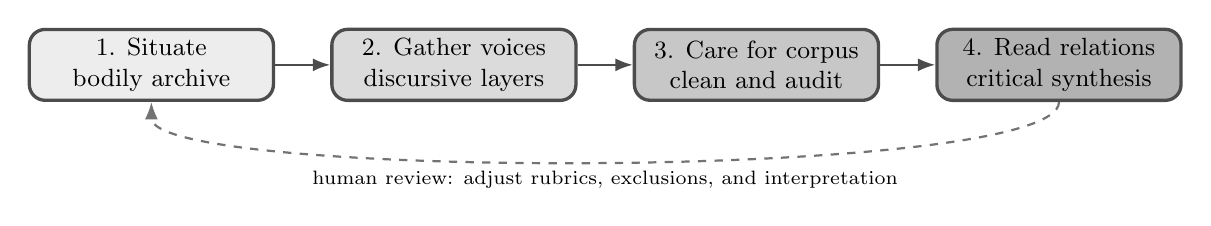
\begin{tikzpicture}[node distance=7mm]
  \node[box, fill=gOne, minimum width=31mm] (a) {1. Situate\\bodily archive};
  \node[box, fill=gTwo, minimum width=31mm, right=of a] (b) {2. Gather voices\\discursive layers};
  \node[box, fill=gThree, minimum width=31mm, right=of b] (c) {3. Care for corpus\\clean and audit};
  \node[box, fill=gFour, minimum width=31mm, right=of c] (d) {4. Read relations\\critical synthesis};
  \draw[arrow] (a) -- (b);
  \draw[arrow] (b) -- (c);
  \draw[arrow] (c) -- (d);
  \draw[softarrow] (d.south) .. controls +(0,-10mm) and +(0,-10mm) .. node[below,font=\scriptsize] {human review: adjust rubrics, exclusions, and interpretation} (a.south);
\end{tikzpicture}%
}
\caption{Interpretive itinerary: the system organizes reading; it does not replace the researcher.}
\label{fig:phases-en}
\end{figure}

\section{Guiding case: tattooing}

For historians, artists, designers, and cultural studies scholars, tattooing
should not be treated as an isolated keyword. It should be divided into
interpretive rubrics:

\begin{table}[H]
\centering
\small
\begin{tabular}{L{0.24\textwidth}L{0.62\textwidth}}
\toprule
\textbf{Rubric} & \textbf{Search variants} \\
\midrule
Core terms & tattoo, tattoos, tatuaje, tatuajes, body art \\
Craft and industry & tattoo artist, tattoo studio, tatuador, tatuadora, artist of tattooing \\
Identity and memory & tattoo meaning, tattoo and identity, tattoo and memory, religious tattoo \\
Society and work & tattoo and youth, tattoo and employment, tattoo discrimination, tattoo and gender \\
Health and regulation & tattoo health, tattoo inks, infection, sanitary regulation \\
Aesthetics and design & tattoo design, traditional tattoo, Mexican tattoo, body ink \\
\bottomrule
\end{tabular}
\caption{Initial rubrics for the tattoo case. Rubrics are editable and must be validated through reading.}
\label{tab:tattoo-rubrics-en}
\end{table}

Exclusions are also declared. They are necessary because \textit{Tatuaje} may
appear as a cigar brand or tattooing may refer to specialized medical
procedures. Excluding terms such as \textit{cigar}, \textit{tobacco},
\textit{robusto}, or \textit{colonoscopic tattooing} does not censor the corpus;
it protects the research question.

\begin{figure}[H]
\centering
\resizebox{\textwidth}{!}{%
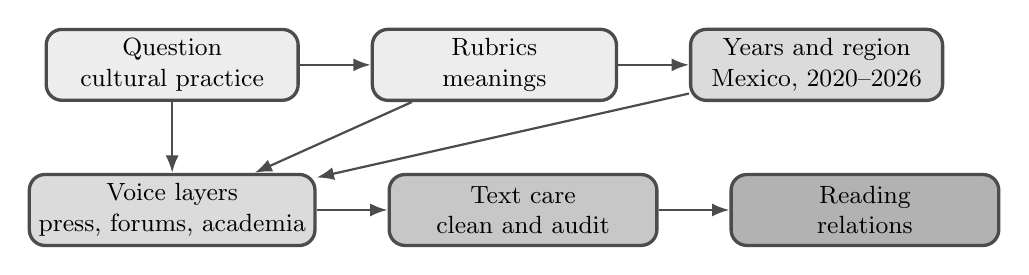
\begin{tikzpicture}[node distance=9mm]
  \node[box, fill=gOne, minimum width=32mm] (q) {Question\\cultural practice};
  \node[box, fill=gOne, minimum width=31mm, right=of q] (r) {Rubrics\\meanings};
  \node[box, fill=gTwo, minimum width=32mm, right=of r] (y) {Years and region\\Mexico, 2020--2026};
  \node[box, fill=gTwo, minimum width=34mm, below=of q] (v) {Voice layers\\press, forums, academia};
  \node[box, fill=gThree, minimum width=34mm, right=of v] (c) {Text care\\clean and audit};
  \node[box, fill=gFour, minimum width=34mm, right=of c] (m) {Reading\\relations};
  \draw[arrow] (q) -- (r);
  \draw[arrow] (r) -- (y);
  \draw[arrow] (q) -- (v);
  \draw[arrow] (r) -- (v);
  \draw[arrow] (y) -- (v);
  \draw[arrow] (v) -- (c);
  \draw[arrow] (c) -- (m);
\end{tikzpicture}%
}
\caption{Corpus design for the tattoo case: notice how the cultural question, meaning rubrics, and voice layers are separated before documents are collected.}
\label{fig:tattoo-corpus-en}
\end{figure}

\section{From documents to narrative traces}

The system saves a separate base for each combination of rubric, year, and
source layer. If a search produces no results, the absence is registered. This
matters: an absence also speaks about the scope of the corpus and about the
limits of collection.

The current collection strategy is sequential and adaptive: it queries the base
term of a rubric first and expands to synonyms only when more evidence is
needed. This reduces pressure on public indexes and preserves the term that
activated each finding. In the tattoo case, collecting through \textit{tatuaje},
\textit{tatuajes}, \textit{tattoo}, or \textit{body art} does not produce the
same corpus; each term carries different communities, languages, and biases.

\begin{table}[H]
\centering
\small
\begin{tabular}{L{0.18\textwidth}L{0.25\textwidth}L{0.42\textwidth}}
\toprule
\textbf{Step} & \textbf{Example} & \textbf{Methodological reading} \\
\midrule
Input & ``tattoo and health'', Mexico, 2021, news & One sense of the topic is located in a public layer. \\
Cleaning & Menus, ads, duplicates, and homonyms are removed & The corpus does not confuse web noise with social narrative. \\
Description & Terms such as ink, skin, regulation, risk appear & These are clues, not conclusions. \\
Relation & Text--actor--idea--source--year & The system shows how voices and concepts are connected. \\
Synthesis & Relevant node: sanitary regulation / tattoo studio & The node becomes an entry point for close reading. \\
\bottomrule
\end{tabular}
\caption{Mini-demonstration of the procedure using the health and regulation rubric.}
\label{tab:mini-demo-en}
\end{table}

\section{Source rights and degrees of evidence}

Extraction must respect the limits of each source. The system does not enter
private spaces, does not automate logged-in sessions, and does not bypass access
restrictions. If a public page allows extraction according to \texttt{robots.txt},
the system attempts to obtain full text. If extraction is not allowed, if the
site only exposes partial material, or if the content is behind a paywall, the
system keeps only a traceable signal: title, snippet, outlet, date, URL, and
source type. That signal may orient the corpus map, but it must not be counted
as equivalent to full textual evidence.

\begin{figure}[H]
\centering
\resizebox{0.98\textwidth}{!}{%
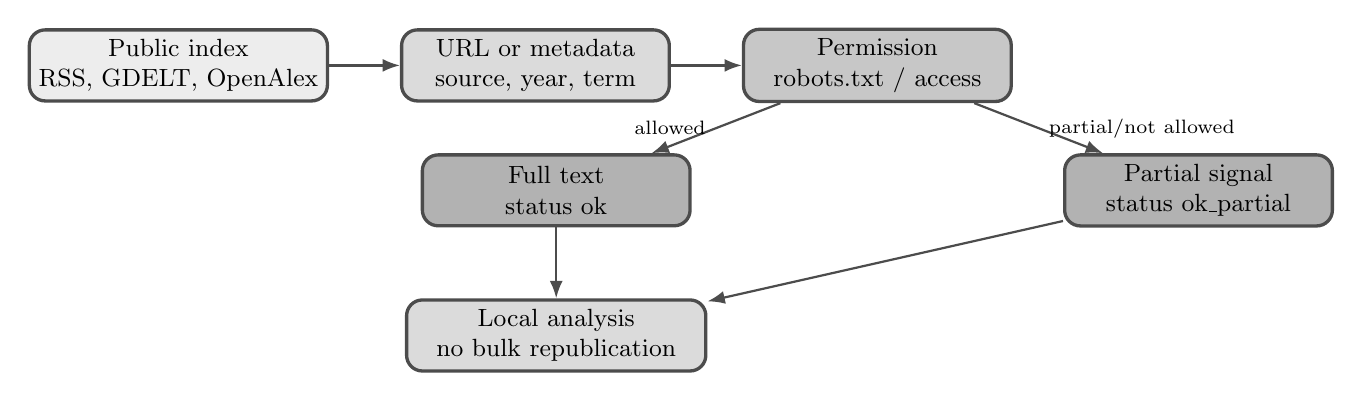
\begin{tikzpicture}[node distance=9mm]
  \node[box, fill=gOne, minimum width=34mm] (i) {Public index\\RSS, GDELT, OpenAlex};
  \node[box, fill=gTwo, minimum width=34mm, right=of i] (u) {URL or metadata\\source, year, term};
  \node[box, fill=gThree, minimum width=34mm, right=of u] (p) {Permission\\robots.txt / access};
  \node[box, fill=gFour, minimum width=34mm, below left=of p] (ok) {Full text\\status ok};
  \node[box, fill=gFour, minimum width=34mm, below right=of p] (parcial) {Partial signal\\status ok\_partial};
  \node[box, fill=gTwo, minimum width=38mm, below=of ok] (local) {Local analysis\\no bulk republication};
  \draw[arrow] (i) -- (u);
  \draw[arrow] (u) -- (p);
  \draw[arrow] (p) -- node[left,font=\scriptsize] {allowed} (ok);
  \draw[arrow] (p) -- node[right,font=\scriptsize] {partial/not allowed} (parcial);
  \draw[arrow] (ok) -- (local);
  \draw[arrow] (parcial) -- (local);
\end{tikzpicture}%
}
\caption{Degrees of evidence: full text and partial signals are stored separately so the corpus does not exaggerate its evidentiary reach.}
\label{fig:rights-evidence-en}
\end{figure}

This distinction is central when studying what people say online. Forums,
public Reddit pages, blogs, and open communities provide traces of public
conversation, but they do not represent the whole social conversation. They
must be read as indexable traces shaped by platform bias, language, moderation,
visibility, and access.

\subsection*{Micro-case for reading}

A publishable run should not stop at document counts. It should show at least
one minimal chain: source, cleaned fragment, assigned label, constructed
relation, and human reading. In the tattoo case, a news item about inks or
sanitary regulation may connect health authorities, tattoo studios, and risk
vocabulary; a forum conversation may connect clients, pain, identity, price, or
trust; an academic article may stabilize medical vocabulary around skin,
infection, or healing.

\begin{table}[H]
\centering
\small
\begin{tabular}{L{0.17\textwidth}L{0.24\textwidth}L{0.23\textwidth}L{0.24\textwidth}}
\toprule
\textbf{Layer} & \textbf{Possible signal} & \textbf{Node/relation} & \textbf{Human reading} \\
\midrule
Press & ``ink regulation'' & health authority--ink--risk & Tattooing appears as a public and sanitary issue. \\
Forum & ``studio recommendation'' & client--tattoo artist--trust & Craft is evaluated through shared experience. \\
Article & ``skin infection'' & skin--procedure--care & The body becomes an object of medical knowledge. \\
\bottomrule
\end{tabular}
\caption{Example of how a document becomes an entry for reading, not an automatic conclusion.}
\label{tab:microcase-en}
\end{table}

\section{Maps of relations}

The narrative network is a map. Each text connects actors, ideas, source, year,
place, and moments of the story. The map does not prove a hypothesis by itself;
it helps decide where close reading should begin.

Actors, ideas, and narrative moments should not be treated as transparent
entities. They may come from local rules, editable dictionaries, n-gram
frequencies, linguistic patterns, and human validation. In a topic such as
tattooing, expected actors may include tattoo artists, clients, health
authorities, physicians, employers, media outlets, and youth collectives; ideas
may group identity, memory, craft, risk, aesthetics, discrimination, or care.
Each assignment must remain correctable through reading.

\begin{figure}[H]
\centering
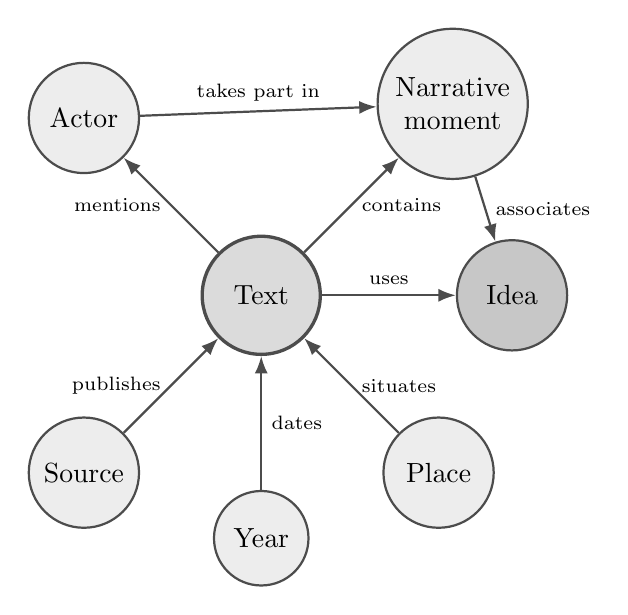
\begin{tikzpicture}[node distance=17mm]
  \node[circle, draw=black!70, very thick, fill=gTwo, minimum size=15mm, align=center] (text) {Text};
  \node[circle, draw=black!70, thick, fill=gOne, above left=of text, minimum size=14mm] (actor) {Actor};
  \node[circle, draw=black!70, thick, fill=gOne, above right=of text, minimum size=17mm, align=center] (moment) {Narrative\\moment};
  \node[circle, draw=black!70, thick, fill=gThree, right=of text, minimum size=14mm] (idea) {Idea};
  \node[circle, draw=black!70, thick, fill=gOne, below left=of text, minimum size=14mm] (source) {Source};
  \node[circle, draw=black!70, thick, fill=gOne, below=of text, minimum size=12mm] (year) {Year};
  \node[circle, draw=black!70, thick, fill=gOne, below right=of text, minimum size=14mm] (place) {Place};
  \draw[arrow] (text) -- node[left,font=\scriptsize] {mentions} (actor);
  \draw[arrow] (text) -- node[right,font=\scriptsize] {contains} (moment);
  \draw[arrow] (text) -- node[above,font=\scriptsize] {uses} (idea);
  \draw[arrow] (source) -- node[left,font=\scriptsize] {publishes} (text);
  \draw[arrow] (year) -- node[right,font=\scriptsize] {dates} (text);
  \draw[arrow] (place) -- node[right,font=\scriptsize] {situates} (text);
  \draw[arrow] (actor) -- node[above,font=\scriptsize] {takes part in} (moment);
  \draw[arrow] (moment) -- node[right,font=\scriptsize] {associates} (idea);
\end{tikzpicture}
\caption{Minimal narrative network: the reader can see what kind of relation is being recorded.}
\label{fig:network-en}
\end{figure}

\section{Exploratory lexical tonality}

Lexical tonality is not interpreted as collective emotion or as the
psychological state of authors. It is used as an exploratory indicator of
evaluative vocabulary. It may show, for example, whether news sources describe
tattooing through risk, whether forums use language of identity, or whether
academic articles concentrate on health and regulation.

The basic indicator compares positive and negative words, with simple rules for
negation and intensification. Results are summarized by year and source layer.
In a radial chart, each axis represents one layer: press, forums, articles, or
reports. Interpretation must always return to textual examples.

\section{Revisable synthesis}

When the map contains too many elements, the system proposes relevant nodes:
actors, ideas, sources, or narrative moments that concentrate relations. This
selection does not replace interpretation. It helps ask which entries deserve
close reading and what relations would be lost if certain nodes were removed.

\begin{figure}[H]
\centering
\resizebox{0.96\textwidth}{!}{%
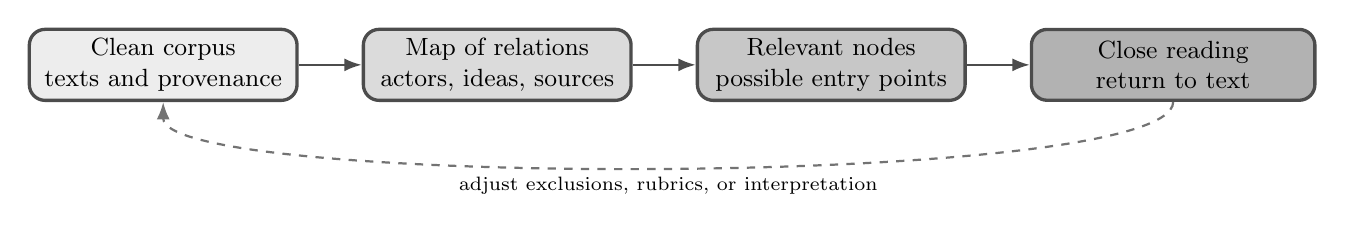
\begin{tikzpicture}[node distance=8mm]
  \node[box, fill=gOne, minimum width=34mm] (corpus) {Clean corpus\\texts and provenance};
  \node[box, fill=gTwo, minimum width=34mm, right=of corpus] (map) {Map of relations\\actors, ideas, sources};
  \node[box, fill=gThree, minimum width=34mm, right=of map] (nodes) {Relevant nodes\\possible entry points};
  \node[box, fill=gFour, minimum width=36mm, right=of nodes] (reading) {Close reading\\return to text};
  \draw[arrow] (corpus) -- (map);
  \draw[arrow] (map) -- (nodes);
  \draw[arrow] (nodes) -- (reading);
  \draw[softarrow] (reading.south) .. controls +(0,-11mm) and +(0,-11mm) .. node[below,font=\scriptsize] {adjust exclusions, rubrics, or interpretation} (corpus.south);
\end{tikzpicture}%
}
\caption{Synthesis is revisable: the algorithm suggests entry points; interpretation returns to the corpus.}
\label{fig:synthesis-en}
\end{figure}

\section{Reproducible output}

The local application exports a structured evidence file that preserves filtered
records, provenance, cleaning decisions, source classification, lexical
tonality, narrative events, actors, idea groups, and maps of relations. For a
stronger publication workflow, a run manifest should also be consolidated with
date, parameters, code version, quotas, seeds, and a fingerprint of the final
corpus.

\section{Limits and biases}

The corpus does not represent a society by itself. It represents a situated
collection of available traces: what indexes find, what platforms allow one to
consult, what media outlets publish, and what certain groups write online. It
may contain biases of language, social class, digital literacy, urban centrality,
source availability, platform moderation, journalistic agenda, and sanitary or
institutional overrepresentation. Exclusions are also interpretive decisions:
removing \textit{colonoscopic tattooing} is reasonable if tattooing is studied
as cultural practice, but it may be wrong if the rubric is medicine or health.
Every exclusion should therefore be registered and justified.

\appendix
\section{Minimal technical note}

The selection of relevant nodes can be formalized as a coverage problem over the
map of relations. The system searches for small sets of nodes that maintain high
interpretive relevance and low structural damage. Operationally, three criteria
are compared: set size, narrative weight of the nodes, and relations that would
be lost if those nodes were removed. The algorithmic details are left in the
appendix because the main question is interpretive: which set of actors, ideas,
or sources offers a defensible entry point for reading the corpus?

\end{document}
